<<<<<<< HEAD
\lecture{4}{16/03/2023}{}

\begin{definition}
    We define the \textbf{superficial degree (or index) of divergence} of the diagram, which determines the degree of ultraviolet divergence ($q \to \infty$) by
    \begin{align*}
        \omega \left( G \right) = L D - 2I
    ,\end{align*}
    with $L = I - V + 1$ as the number of independent integration variables/loops, $D$ is the dimension and $I$ is the number of internal lines.
\end{definition}

This is motivated by the general dimensional form of the integrand, namely,
\begin{align*}
    \int^{\Lambda} \left( \dd{^{D}q} \right)^{L} \left( p^2 \right)^{-I}
,\end{align*}
has dimension $\omega \left( G \right) $.

If $\omega \left( G \right) > 0$ then the integral diverges with $\Lambda^{\omega \left( G \right) } \left( \ln \Lambda \right)^{n}$ for $n \in \Z$. Similarly, if $\omega\left( G \right) = 0$ then the integral diverges with $\left( \ln \Lambda \right)^{p}$. Lastly, if $\omega \left( G \right) < 0$ then we call the graph \textbf{superficially convergent} (as sub-integrations could still diverge).

\subsection{Topological Argument}

Alternative expressions for $\omega \left( G \right) $ prove useful.

For general derivative type interactions, our dimension now scales with
\begin{align*}
    \omega \left( G \right) &= LD - 2 I + \sum_{i=1}^{V} \delta_{i} 
    \intertext{where our $i$ interactions each contains $\delta_i$ derivatives. With $L = I - V + 1$, we have}
    \omega \left( G \right) &= I \left( D - 2 \right) - VD + D + D + \sum_{i=1}^{V} \delta_i    \\
    \omega \left( G \right) - D &= I \left( D-2 \right) + \sum_{i=1}^{V} \left( \delta_i - D \right)  \\
    \intertext{Splitting $n_i = n_i^{\text{int}} + n_i^{\text{ext}}$ we have $I = \frac{1}{2} \sum_{i}^{} n_i^{\text{int}} $ and thus}
    \omega \left( G \right) - D &= \left( \frac{D}{2} - 1 \right) \sum_{i}^{} n_i^{\text{int}} + \sum_{i}^{} \left( \delta_i - D \right)    \\
    \omega \left( G \right) - D &= \left( \frac{D}{2} - 1 \right) \sum_{i}^{} \left( n_i - n_i^{\text{ext}} \right)  + \sum_{i}^{} \left( \delta_i - D \right)    \\
    \intertext{Defining $\omega_i = n_i \left( \frac{D}{2} - 1 \right) + \delta_i$ we see with $E = \sum_{i}^{} n_i^{\text{ext}}$ we have}
    \omega \left( G \right) - D &= \sum_{i}^{} \left( \omega_i - D \right)  = E \left( \frac{D}{2} - 1 \right) 
,\end{align*}

\begin{examples}
    For $\phi^{4}$ theories,
    \begin{align*}
        \omega_i &= 4 \left( \frac{D}{2} - 1 \right) + 0  \\
        &= 2D - 4 \\
        \implies \omega \left( G \right) - D &= V \left( 4\frac{D}{2} - 4 - D \right) - E \left( \frac{D}{2} -1 \right)  \\
        &= V \left( D - 4 \right) - E \left( \frac{D}{2} -1 \right)    \\
        \intertext{For $E = 2$}
       \omega \left( G \right)  &= V \left( D - 4 \right) + 2 \\
        \intertext{For $E = 4,$}
       \omega \left( G \right) &= V \left( D - 4 \right) + 4 - D \\
       \intertext{For $E = 6,$}
       \omega \left( G \right) &= V \left( D - 4 \right) + 6 - 2D
    .\end{align*}
    Namely, as the number of external lines rises $\omega \left( G \right) $ decreases. For such a $\phi^{4}$ theory with $D = 4$, we see that only $E < 6$ are superficially divergent.
\end{examples}

\subsection{Dimensional argument}

We can write a general interaction term as
\begin{align*}
    g_i \int \dd{^{D}x} \grad^{\delta_i} \phi^{n_i}
,\end{align*}
which must be dimensionless, and thus
\begin{align*}
    \left[ g_i \right] - D + \delta_i + n_i \left[ \phi \right] &= 0
    \intertext{where $\left[ \phi \right] = \frac{D}{2} - 1$. Using the $\omega_i$ index definition above, we can write the dimension of the coupling constant as}
    \left[ g_i \right] &= D - \omega_i
.\end{align*}
One can recover the previous result from this expression by considering $\Gamma^{\left( E \right) }\left( k \right) $.


\subsection{Infrared divergences}

While ultraviolet divergences occur independently of the external momenta as they are concerned with internal propagators, \textbf{infrared divergences} can arise due to unconstrained external momenta.

\begin{figure}[h]
    \centering
    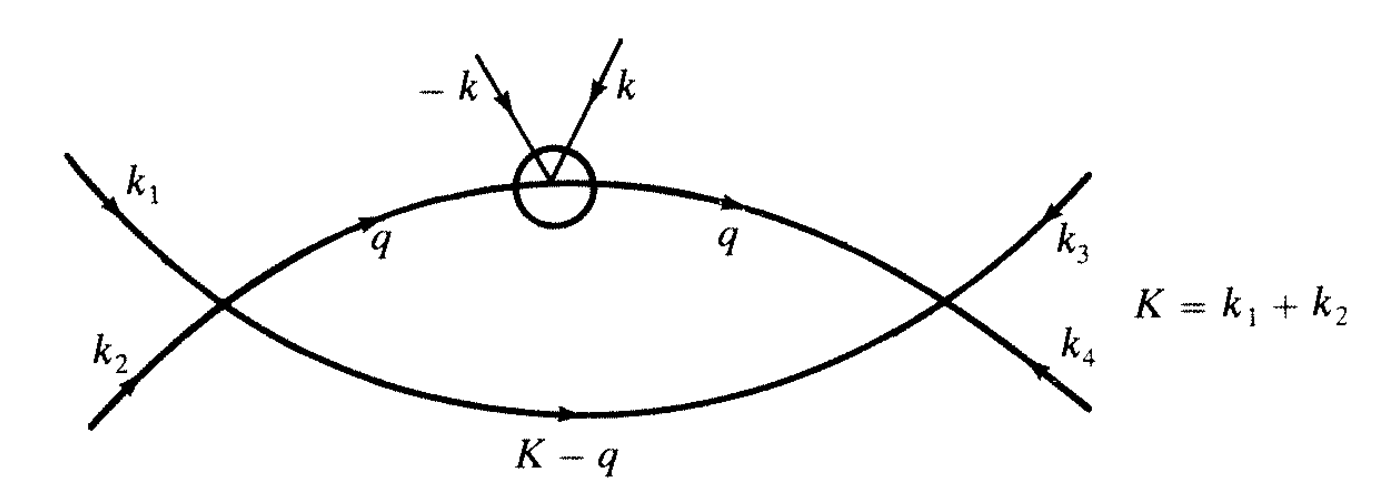
\includegraphics[width=0.8\textwidth]{figures/5.32.png}
    \caption{5.32 from LeBellac p.g. 193}
    \label{fig:5.32}
\end{figure}

Figure \ref{fig:5.32} is proportional to
\begin{align*}
    \int \frac{\dd{^{4}q}}{q^{4} \left( k - q \right)^{4}}
,\end{align*}
which diverges for small $q \to 0$, namely, in the infrared.

\begin{definition}
    A configuration of external momenta is called \textbf{non-exceptional} if no partial sum of the $k_i$ vanishes,
    \begin{align*}
        \sum_{i\in I}^{} k_i \neq 0 
    ,\end{align*}
    for any subset $I$ of the external momenta. Likewise, it is called \textbf{exceptional} if any partial sum vanishes.
\end{definition}

In a non-exceptional configuration, all external momenta can be linked by internal lines with nonzero momentum which we call \textbf{hard lines}. 

If this was not the case, then we could split the diagram into two by cutting internal lines of zero momentum, appropriately named \textbf{soft lines}.

If we contract all hard internal lines to a single vertex, and set $n$ to be the number of soft internal lines, we have the relations
\begin{align*}
    L &= I - V \\
    2I &= 4 V + n \\
    \intertext{which yields a superficial divergence of}
    \omega \left( G \right) = n + L \left( D - 4 \right) 
,\end{align*}
if all internal loops have negligible momenta.

Namely, we have that the diagram is infrared-convergent when $D = 4$ as we have $n \geq 2 \implies \omega \left( G \right) > 0$.

On the contrary, for $D < 4$, diagrams are commonly infrared divergent even in non-exceptional configurations.

\begin{theorem}[ (Weinberg's Theorem)]
    Consider a $\phi^{4}$ theory in $D = 4$ and assume that $J$ is ultraviolet convergent. If its $m = 0$ limit exists, as it will if the diagram is non-exceptional, then
    \begin{align*}
        J\left( \lambda k_i \right) \underset{\lambda \to \infty}{\sim} \lambda^{\omega \left( G \right) }
    .\end{align*}
    If $J$ has to be renormalized due to ultraviolet divergences, then we find that
    \begin{align*}
        J\left( \lambda k_i \right) \underset{\lambda \to \infty}{\sim} \lambda^{\omega \left( G \right) }\left( \ln \lambda \right)^{n}
    ,\end{align*}
    for some fixed $n \in \Z$ determined by the graph.
\end{theorem}

\subsection{Classification of Renormalizability}

The systematic removal of such divergences is called \textbf{renormalization}. In general, this is done by \textit{absorbing} the divergences into the definition of the coupling constant, mass and field normalization.

For a interaction with only a single field, the superficial degree of divergence of a graph $G$ reduces to
\begin{align*}
    \omega \left( G \right) - D &= V \left( \omega - D \right) - E \left( \frac{D}{2} - 1 \right)  \\
,\end{align*}
where $D - \omega = \left[ g \right] $ is the dimension of the coupling constant.
Clearly, we can see that if $\omega > D$, then the degree of divergence increases as $V$ (or equivalently the order of the perturbation) increases. Such a theory is \textbf{nonrenormalizable}. We would need to fix infinitely many parameters in order to see finite results. It is possible to have nonrenormalizable interactions in some cases where the divergences cancel for all physical quantities, but this is equivalent to a renormalizable theory.

If $\omega < D$ then we will only have a finite number of divergent graphs as for sufficiently large $V$, $\omega \left( G \right) < 0$. Such theories are called super-renormalizable and despite their appeal, are challenging and have yet to find application.

Lastly, if $\omega = D$ then the degree of divergence is independent of the order of the perturbation and $\left[ g \right] = 0$. Such theories are \textbf{renormalizable}. We can fix the divergence by fixing a finite number of parameters.

\begin{example}
    For a $\phi^{4}$ theory, $\omega_i = 2D - 4$, and thus
    \begin{align*}
        \left[ g_0 \right] &= 4 - D
    .\end{align*}
\end{example}

where if $D = 4$ the theory is renormalizable and thus we find that only the two-point and the four-point correlation functions are divergent. For $E \geq 6$ the correlation functions are superficially convergent. Subintegrations can ruin this visage, however we have the following theorem to help.

\begin{theorem}[ ( First convergence theorem)]
    If all connected 1-PI subdiagrams $\gamma$ of a diagram $G$ including itself are such that $\omega \left( \gamma \right) < 0$, then the Feynman integral of $G$ is absolutely convergent.
\end{theorem}

\subsection{Regularization}

There are a number of ways to regularise integrals, namely, to make them finite in the process of a calculation. Note that regularization procedures may differ but should all produce the same renormalized theory.


We have the following common regularization procedures:
\begin{enumerate}[label=\alph*)]
    \item Brute-force cutoff: restricting integrals to $\left\|\vb{q}\right\| < \Lambda$. This is impractical beyond one-loop.
    \item Schwinger regularization which follows from
        \begin{align*}
            \frac{1}{q^2 + m^2} \to \int_{\Lambda^{-2}}^{\infty} \dd{\alpha} e^{-\alpha \left( q^2 + m^2 \right) }
        .\end{align*}
    \item Pauli-Villars regularisation which follows from
        \begin{align*}
            \frac{1}{q^2 + m^2} \to \frac{1}{q^2 + m^2 } - \frac{1}{q^2 + \Lambda^2}
        .\end{align*}
    \item Dimensional regularization where we take $\dd{q}^{4- \epsilon}$
    \item and lattice regularization where we quantize space and replace fields by a lattice variable
        \begin{align*}
            \phi_i \simeq \frac{1}{a^{D}} \phi \left( x \right) \dd{^{D}x}
        ,\end{align*}
        where we integrate over a volume $a^{D}$ centered on site $i$ with a cutoff $\Lambda \sim  \pi/a$.
\end{enumerate}

Some regularization procedures break symmetries, e.g. lattice regularization breaks rotation and translational invariance.

However, even in this case we can show that the resulting renormalized theory does have the previous symmetries even if they were not present through every step of the calculation.

There also exists cases where the classical symmetry cannot be preserved and this is what is called an \textbf{anomaly}.





=======
\lecture{3}{17/03/2023}{}

\subsection{5.6}
For an integral that behaves like:
\begin{align*}
    \int^{\Lambda}q^{\omega(G)-1}\dd q
\end{align*}
We can define the superficial degree of divergence for an integral over q %TODO
\begin{equation*}
    \omega(G)=LD-2I
\end{equation*}
The integral is divergent for $\omega(G)>\geq0$ and superficially convergent for $\omega(G)<0$, meaning that integration over a subset of the domain may not converge.
It is possible to derive an expression for this superficial degree in terms of the number of external lines of the diagram.
\\

\subsubsection{Topological argument}
Consider an interaction permitting various powers of $\phi$ and its derivatives eg. $\phi(\nabla\phi)^2$.
From Wick's theorem:
\begin{align*}
    \overline{\phi(x)\nabla\phi(z)}\rightarrow\nabla_z G_0(x-z)=F[ikG_0(k)]
\end{align*}
Where $F[g]$ denotes the Fourier transform of $g$. Thus the derivative has the effect of multiplying the the vertex by a factor of $ik$.
>>>>>>> a703dc1b47d6bc29e58b9b310857046a015d204b

